\def\mytitle{LINE USING PYTHON}
\def\myauthor{Mukesh Guptha.CH}
\def\contact{mukeshchinta1313@gmail.com}
\def\mymodule{Future Wireless Communication (FWC)}
\documentclass[10pt, a4paper]{article}
\usepackage[a4paper,outer=1.5cm,inner=1.5cm,top=1.75cm,bottom=1.5cm]{geometry}
\twocolumn
\usepackage{graphicx}
\graphicspath{{./images/}}
\usepackage[colorlinks,linkcolor={black},citecolor={blue!80!black},urlcolor={blue!80!black}]{hyperref}
\usepackage[parfill]{parskip}
\usepackage{lmodern}
\usepackage{tikz}
	\usepackage{physics}
%\documentclass[tikz, border=2mm]{standalone}
\usepackage{karnaugh-map}
%\documentclass{article}
\usepackage{tabularx}
\usepackage{circuitikz}
\usetikzlibrary{calc}
\usepackage{amsmath}
\usepackage{amssymb}
\renewcommand*\familydefault{\sfdefault}
\usepackage{watermark}
\usepackage{lipsum}
\usepackage{xcolor}
\usepackage{listings}
\usepackage{float}
\usepackage{titlesec}
\providecommand{\mtx}[1]{\mathbf{#1}}
\titlespacing{\subsection}{1pt}{\parskip}{3pt}
\titlespacing{\subsubsection}{0pt}{\parskip}{-\parskip}
\titlespacing{\paragraph}{0pt}{\parskip}{\parskip}
\newcommand{\figuremacro}[5]{
    \begin{figure}[#1]
        \centering
        \includegraphics[width=#5\columnwidth]{#2}
        \caption[#3]{\textbf{#3}#4}
        \label{fig:#2}
    \end{figure}
}
\newcommand{\myvec}[1]{\ensuremath{\begin{pmatrix}#1\end{pmatrix}}}
\let\vec\mathbf
\lstset{
frame=single, 
breaklines=true,
columns=fullflexible
}

\title{\mytitle}
\author{\myauthor\hspace{1em}\\\contact\\FWC22069\hspace{6.5em}IITH\hspace{0.5em}\mymodule\hspace{6em}ASSIGN-4}
\date{}
\begin{document}
	\maketitle
 \paragraph*{\large Problem Statement}
$-$ \textbf{ Find the equation of the line passing through  (-3,5) and perpendicular to the line through the points (2,5) and (-3,6).}
 
\begin{figure}[h]
\centering
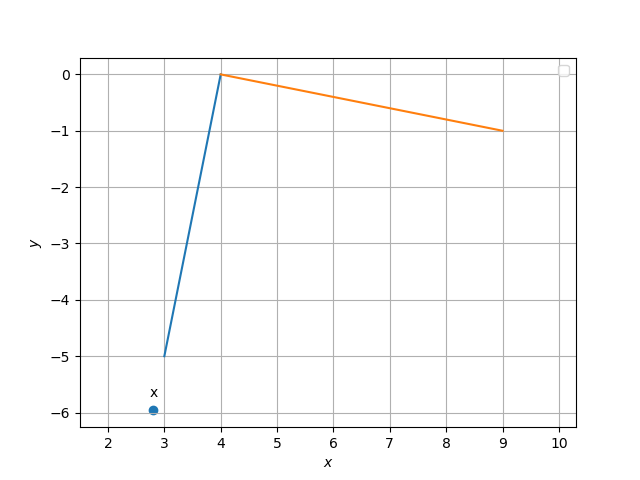
\includegraphics[width=1\columnwidth]{Figure_1.png}
\caption{perpendicular intersection}
\end{figure}
	\section*{Construction}
\vspace{2mm}
 the input parameters are as follows
{
\setlength\extrarowheight{4pt}
 
 \begin{tabular}{|c|c|c|}
	\hline
	\textbf{Symbol}&\textbf{Value}&\textbf{Description}\\
	\hline
 c&$
	\begin{pmatrix}
		5\\
		-1\\
	\end{pmatrix}$
	&coefficients of line \\
	\hline
 d&$
	\begin{pmatrix}
		20\\
	\end{pmatrix}$
	&constants\\
	\hline
 \end{tabular}
}
\section*{\large solution}

\subsection*{\large part 1}
let us take A=(2,5),B=(-3,6) and P=(-3,5).Directional vector  of the points\vspace{4mm}m=B-A\\
\begin{equation}
m=\begin{pmatrix}
    2\\
    5\\
\end{pmatrix}-\begin{pmatrix}
    -3\\
    6\\
\end{pmatrix}\hspace{2em}
m=\begin{pmatrix}
    5\\
    -1\\
\end{pmatrix}
\label{eq-1}
\end{equation}


\begin{eqnarray}
\vec{m^t\vec{(X-P)}}=0
\end{eqnarray}
\begin{equation}
\begin{pmatrix}
    5 &-1\\
\end{pmatrix}\begin{pmatrix}
    X-P\\
\end{pmatrix}
    \label{eq-3}
\end{equation}

\begin{equation}
 \begin{pmatrix}
    5 & -1\\
\end{pmatrix}\begin{pmatrix}
    x+3\\
    y-5\\
\end{pmatrix}
\label{eq-4}
\end{equation}
The required line equation is 
\begin{equation}
 5\vec{x}-\vec{y}+20=0
\label{eq-5}
\end{equation}
\end{document}